%% 
%% Copyright 2007, 2008, 2009 Elsevier Ltd
%% 
%% This file is part of the 'Elsarticle Bundle'.
%% ---------------------------------------------
%% 
%% It may be distributed under the conditions of the LaTeX Project Public
%% License, either version 1.2 of this license or (at your option) any
%% later version.  The latest version of this license is in
%%    http://www.latex-project.org/lppl.txt
%% and version 1.2 or later is part of all distributions of LaTeX
%% version 1999/12/01 or later.
%% 
%% The list of all files belonging to the 'Elsarticle Bundle' is
%% given in the file `manifest.txt'.
%% 

%% Template article for Elsevier's document class `elsarticle'
%% with numbered style bibliographic references
%% SP 2008/03/01

%\documentclass[preprint,12pt]{elsarticle}
\documentclass[final,3p,times,review]{elsarticle}

%% Use the option review to obtain double line spacing
%% \documentclass[authoryear,preprint,review,12pt]{elsarticle}

%% Use the option review to obtain double line spacing
%% \documentclass[authoryear,preprint,review,12pt]{elsarticle}


% Add Reference title
\def\bibsection{\section*{References}}
% NOMENCLATURE
%\usepackage{framed} % Framing content
%\usepackage{multicol} % Multiple columns environment
%
%\usepackage{nomencl} % Nomenclature package
%\makenomenclature
%\setlength{\nomitemsep}{-\parskip} % Baseline skip between items
%
%\renewcommand*\nompreamble{\begin{multicols}{2}}
%\renewcommand*\nompostamble{\end{multicols}}

%% Use the options 1p,twocolumn; 3p; 3p,twocolumn; 5p; or 5p,twocolumn
%% for a journal layout:
%% \documentclass[final,1p,times]{elsarticle}
%% \documentclass[final,1p,times,twocolumn]{elsarticle}
%% \documentclass[final,3p,times]{elsarticle}
%% \documentclass[final,3p,times,twocolumn]{elsarticle}
%% \documentclass[final,5p,times]{elsarticle}
%% \documentclass[final,5p,times,twocolumn]{elsarticle}

%% For including figures, graphicx.sty has been loaded in
%% elsarticle.cls. If you prefer to use the old commands
%% please give \usepackage{epsfig}

%% The amssymb package provides various useful mathematical symbols
\usepackage{amssymb}
%% The amsthm package provides extended theorem environments
%% \usepackage{amsthm}

%%%%%%%%%%%% PACKAGE TO MAKE DOTTED LINES %%%%%%%%%%%%%%%%%%%%%%%%%%%%%%%%%%
\usepackage{array,arydshln}
%\setlength\dashlinedash{0.2pt}
%\setlength\dashlinegap{4.5pt}
%\setlength\arrayrulewidth{0.2pt}
%%%% Another combination of values
\setlength\dashlinedash{0.2pt}
\setlength\dashlinegap{1.5pt}
\setlength\arrayrulewidth{0.3pt}

%%%%%%%%%%%%%%% PACKAGE TO INCREASE THICKNESS OF TABLE ROW %%%%%%%%%%%%%%%%%%%%
\usepackage{array}
\usepackage{todonotes}


\newcolumntype{M}[1]{>{\centering\arraybackslash}m{#1}}
\newcolumntype{N}{@{}m{0pt}@{}}

%%%%%%%%%%% FOR BETTER REFERENCES %%%%%%%%%%%%%%%%%%%%%%%%
\usepackage[nodots]{numcompress}
\biboptions{square,sort&compress}
%%%%%%%%%%% TABLE DIMENSION %%%%%%%%%%%%%%%%%%%%%%%%
\usepackage{tabularx}

%%%%%%%%%%% LANDSCAPE %%%%%%%%%%%%%%%%%%%%%%%%
\usepackage{lscape}

\usepackage{amsmath}
\usepackage{amssymb}
%%%%%%%%%%%%%%%%%%%%%%%%%%%%%%%%%%%%%%%%%%%%%%%%%%%%%%%%%%%%%%%%%%%%%%%%%%%%

%% The lineno packages adds line numbers. Start line numbering with
%% \begin{linenumbers}, end it with \end{linenumbers}. Or switch it on
%% for the whole article with \linenumbers.
\usepackage{lineno}

\usepackage{graphicx,psfrag,subcaption,booktabs}

\usepackage{caption}

\usepackage{url}

%%%%%%%%%%% PACKAGE FOR CHECK MARKS %%%%%%%%%%%%%%%%%%%%%%%%
\usepackage{tikz}
\def\checkmark{\tikz\fill[scale=0.4](0,.35) -- (.25,0) -- (1,.7) -- (.25,.15) -- cycle;} 

\journal{SolarEnergy}

\begin{document}
\linenumbers
\modulolinenumbers[1]
\begin{frontmatter}

%% Title, authors and addresses

%% use the tnoteref command within \title for footnotes;
%% use the tnotetext command for theassociated footnote;
%% use the fnref command within \author or \address for footnotes;
%% use the fntext command for theassociated footnote;
%% use the corref command within \author for corresponding author footnotes;
%% use the cortext command for theassociated footnote;
%% use the ead command for the email address,
%% and the form \ead[url] for the home page:
%% \title{Title\tnoteref{label1}}
%% \tnotetext[label1]{}
%% \author{Name\corref{cor1}\fnref{label2}}
%% \ead{email address}
%% \ead[url]{home page}
%% \fntext[label2]{}
%% \cortext[cor1]{}
%% \address{Address\fnref{label3}}
%% \fntext[label3]{}

\title{Steady-state and dynamic validation of a parabolic through collector model using the ThermoCycle Modelica library}

%% use optional labels to link authors explicitly to addresses:
%% \author[label1,label2]{}
%% \address[label1]{}
%% \address[label2]{}

%\author{Adriano Desideri, Martin van den broek, Gusev Sergei, Vincent Lemort, Sylvain Quoilin}
% Define authors %
%\fnref{fn1}}
\author[rvt]{Adriano Desideri\corref{cor1}}
\ead{adesideri@ulg.ac.be}
\cortext[cor1]{Corresponding author}
\author[rvt]{Remi Dickes}
\author[focal]{Javier Bonilla}
\author[focal]{Loreto Valenzuela}
\author[rvt]{Sylvain Quoilin}
\author[rvt]{Vincent Lemort}
\address[rvt]{Thermodynamics laboratory, University of Li\`ege,
Campus du Sart Tilman, B49, B-4000 Li\`ege, Belgium}
\address[focal]{PSA-CIEMAT, Plataforma Solar de Almer\' ia - Centro de Investigaciones Energ\' eticas, MedioAmbientales y Tecnológicas, Crta. de Sen\' es s/n, 04200, Tabernas (Almer\' ia), Spain}
%
%
%
%
%
%
%
%
%
\address{}
%
\begin{abstract}
%% Text of abstract
Small-capacity  ($<200$ kW$_\mathrm{el}$)  concentrated solar power plants has been recognized as a promising  technology for micro power applications. In particular, parabolic through collectors have been identified as the most promising focusing technology. In this context, physics-based dynamic model of parabolic through constitutes a significant tool for the further development of the technology, allowing to evaluate and optimize response times during transients, or to implement and test innovative control strategies. In this contribution, the dynamic model of a parabolic trough line based on the ThermoCycle Modelica library is validated against steady-state and transient experimental results from the parabolic through test loop available at the Plataforma Solar de Almer\'ia, Spain. The simulation results are in good agreement with the measurements, both in steady-state and in transient conditions. The validated model is readily usable to investigate demanding dynamics-based problems for low capacity solar power systems.
\end{abstract}
%
\begin{keyword}
%% keywords here, in the form: keyword \sep keyword
Parabolic through collectors, Dynamic validation, Modelica
%% PACS codes here, in the form: \PACS code \sep code

%% MSC codes here, in the form: \MSC code \sep code
%% or \MSC[2008] code \sep code (2000 is the default)

\end{keyword}

\end{frontmatter}

%% \linenumbers

%% main text
\section{Introduction}
\label{Intro}

%%%%%%%%%%%%%%%%%%%%%%%%%%%%%%%% NOMENCLATURE %%%%%%%%%%%%%%%%%%%%%%%%%%%%%%%%

\begin{table}[h!]
\begin{tabular}{lp{7.5cm}}
\textbf{Nomenclature}\\
\textit{Acronyms} \\
CSP & Concentrated solar power\\
PTC & Parabolic through collectors\\
ORC & Organic Rankine cycle\\
HTF & Heat transfer fluid\\
DSG & Direct steam generation\\
FV  & Finite volume \\
MB & Moving boundary \\
PSA & Plataforma solar de Almer\' ia \\
HCE & Heat collection element \\
CV & Control volume \\
TT & Temperature transmittance \\
DNI & Direct normal irradiation \\
ETC & EuroTrough collector \\
SF & Solar field \\
EI & Exogenous inputs \\
IAM & Incidence angle modifier \\
PCE & Percentage computational effort \\
\textit{Subscripts} \\
su  & supply \\
ex & exhaust \\
conv & convection \\
amb & ambient \\
\end{tabular}
\begin{tabular}{lp{7.5cm}}
sol  & solar\\
rad & radiation\\
ext & external\\
int & internal \\
meas & measured \\
el & electrical \\
wf & working fluid \\
\textit{Symbols} \\
$p$ & pressure (bar)\\
$T$ & temperature ($^{\circ}$C)\\
$V_\mathrm{s}$ & volume (m$^3$)\\
$\dot{q}$& heat flux (kW.m$^{-2}$) \\
$M$ & mass (kg)\\
$h$ & specific enthalpy (kJ.kg$^{-1}$)\\
$\rho$ & density (kg m$^{-3}$)\\
$\dot{m}$& mass flow (kg.s$^{-1}$) \\
$ C_\mathrm{p} $& specific heat capacity (kJ.(kg.K)$^{-1}$) \\
$A$ & area (m$^{2}$)\\
$D$ & diameter (m)\\
$N$ & number of nodes (-)\\
$\bar{\varepsilon}$ & relative error (\%)\\
$E$ & energy  (kJ)\\
%$\epsilon$ & percentage relative error\\
%$N_c$ & number of cells \\
\end{tabular}
\end{table}
 %%%%%%%%%%%%%%%%%%%%%%%%%%%%%%%% END NOMENCLATURE %%%%%%%%%%%%%%%%%%%%%%%%%%%%%%%%
%
Recent studies have envisaged the potential of small-capacity ($<200$ kW$_\mathrm{el}$) concentrated solar power (CSP) plants in case the future distributed energy scenario is considered \cite{Casati2012a,Prabhu2006}. The first documented CSP systems date back to the end of the 10$^\mathrm{th}$ century \cite{Butti_1980}. Several CSP systems were developed and tested during the years, and the first commercial plants were built in the 80's in California, USA \cite{IRENA_CSP_2013}.  The main collector technologies are point-focus sing parabolic dishes, solar towers, and line-focussing parabolic troughs, vacuum tube or non-concentrating flat plate collectors \cite{Winter1991}. Non or low-concentrating configurations are particularly attractive for small-scale power units, as the lower investment costs may lead to economic viability. In particular,  parabolic through collectors (PTCs) are suited to supply low or medium temperature thermal energy to generate electricity in combination with low-temperature organic Rankine cycle (ORC) engines \cite{Verneau1978,Angelino1984Areview}.\\

PTCs are by far the most mature solar concentrating technologies, as demonstrated commercially \cite{Fernandez_Garcia2010}. 
 A PTC is a line-focusing  parabola-shaped mirror which concentrates direct solar radiation on the absorber tube, located in the parabola's focal line. An heat transfer fluid (HTF) is pumped through the absorber tube acquiring thermal energy from the concentrated solar radiation. Parabolic trough solar thermal power plants commonly use thermal oil as HTF. This technology has been continuously improved since its first commercial implementation \cite{Canada_Saguaro_2005}. In recent years, water has been tested as HTF in the collectors. The technology, called Direct Steam Generation (DSG),  generates  superheated steam directly from the collectors and presents important challenges due to phase changes in the HTF \cite{Bonilla_MB_2015}.\\

Due to the non-constant nature characterizing the direct solar irradiation, specific control strategies ensuring safe and optimal operation of the CSP systems in any conditions are required. Before a control system can be designed, the dynamic behaviour of the CSP plant must be investigated.
To this end,  it is fundamental to study the transient related to the solar field. In the literature,  dynamic process models of PTCs are mainly one-dimensional in flow direction and date back to the late ’70s. The Finite Volume (FV) method is the preferred approach for the discretization of the absorber tube. Nevertheless, when DSG is considered Moving Boundary (MB) models can be also applied.\\

Ray \cite{Ray1981} presented in 1980 a non-linear dynamic model of a parabolic trough unit for DSG. The FV modelling approach was adopted and the transient response of the model under different step disturbances was presented as typical results. Hirsch et al. \cite{Hirsch2005,Eck2007} developed one of the first Modelica PTC models.  A FV based solar collector model of a DSG plant was introduced together with a preliminary validation based on the first experimental results of the DISS facility at the Plataforma Solar de Almer\'ia (PSA), Spain. More recently, a tri-dimensional non-linear dynamic thermohydraulic model of a PTC was also developed in Modelica and coupled to a solar industrial process heat plant modelled in TRNSYS \citep{Silva2013}. A DSG PTC model was validated against results from the DISS facility, in \cite{Lobon2014}, showing a good agreement. Several dynamic models of CSP plants were developed in Modelica based on the ThermoSysPro library \citep{Hefni2014}.  A full scale dynamic model of a parabolic trough power plant with a thermal storage system is presented in \cite{Almaliki2016_1}; simulation results are compared to experimental data from the real power plant.
This work is extended in \cite{Almaliki2016_2} including the power block and all the automation processes, simulated results are compared to measured data from an existing solar power plant. A simulation model for DSG in PTCs is developed in TRNSYS \cite{Biencinto2016}, results are validated with real data at the DISS facility. A thermal hydraulic RELAP5 DSG PTC model was validated against the DISS facility in \cite{Serrano2017}, a new experimental correlation for heat losses was also provided. A non-linear dynamic model of once-through DSG PTCs was developed in \citep{Guo2017}, transfer functions of outlet fluid temperature and mass flow rate were also derived.\\

The present work focuses on the steady-state and dynamic validation of a parabolic through collector model included in the open-source ThermoCycle Modelica library, for the modelling of small thermo-hydraulic system \cite{Quoilin2014a}. The main contribution consists in a through validation of the PTC model against experimental data collected at the PTTL facility in Almer\'ia, Spain. 
The model is a detailed implementation of the Forristal approach \citep{Forristal2003}, it is highly customizable and can be used to model any kind of PTC solar field.
The paper is organized as follows: section~\ref{Sec:DynModel} presents the PTC model in detail. Section~\ref{Sec:Measurements} details the experimental campaign. Section~\ref{Sec:Validation} report the results for the steady-state and dynamic validation analysis. Section~\ref{Sec:Disccusion} discusses critical aspects when modelling parabolic through collectors. Finally, section~\ref{Sec:Conclusions} draws the main conclusions of this work.
%
\section{Parabolic trough collector modelling}
\label{Sec:DynModel}

The parabolic trough model is developed in the Modelica language~\cite{Elmqvist1978} and is part of the open-source ThermoCycle library ~\cite{Quoilin2014a}. As depicted in Figure~\ref{fig:PTC_FV}, the model relies on a finite-volume approach for the modelling of the heat collection element (HCE), which is discretized along its axial axis in $N$ constant and uniform control volumes (CV). The one-dimensional modelling method is justified by the large ratio between the diameter and the length of the HCE. 
%
\begin{figure}[h]
	\centering
	\begin{subfigure}[b]{0.48\textwidth}
		\centering
		\includegraphics[width=0.95\textwidth]{Figures/PTC_FV.pdf}
		\caption{}
		\label{fig:PTC_FV}	
	\end{subfigure}
	\begin{subfigure}[b]{0.48\textwidth}
		\centering
		\includegraphics[width=0.7\textwidth]{Figures/PTC_GUI}
		\caption{}
		\label{fig:PTC_GUI}
	\end{subfigure}
	\caption{Parabolic trough collector model in ThermoCycle. \ref{fig:PTC_FV}: One-dimensional finite-volume modelling of the PTC. \ref{fig:PTC_GUI}: Object diagram of the solar collector model from the GUI of Dymola.}
	\label{fig:PTC_model}
\end{figure}
%
Following the object-oriented formalism of Modelica, the PTC model is built by interconnecting two sub-components, i.e. the \textit{Flow1D} and the \textit{SolAbs} models. These two are linked together through a thermal port as depicted in Figure~\ref{fig:PTC_GUI}.\\

The \textit{Flow1D} component simulates the fluid flow in the HCE. In each CV, both mass and energy balances are solved assuming an incompressible fluid and a static momentum balance. Considering the above mentioned assumptions, the final conservation law formulations for each CV are reported in Equations \ref{eq:MassBalance} to \ref{eq:MomentumBalance}, with pressure, $p$, and specific enthalpy, $h$, as dynamic state variables.
%
\begin{align}
\label{eq:MassBalance}
\frac{dM}{dt} & = \dot{m}_{su}-\dot{m}_{ex} = 0  \quad \text{with} \quad
\frac{dM}{dt} = V \left( \frac{\partial \rho}{\partial h}  \cdot \frac{dh}{dt} + \frac{\partial \rho}{\partial p} \cdot \frac{dp}{dt} \right) \\
\label{eq:EnergyBalance}
V\rho \frac{dh}{dt} & = \dot{m}_{su}(h_{su} - h) - \dot{m}_{ex}(h_{ex} - h) + V \frac{dp}{dt} + A \cdot \dot{q}_{conv,fl} \\
\label{eq:MomentumBalance}
p_{su} & = p_{ex}
\end{align}
%
The ''su'' (supply) and ''ex'' (exhaust) subscripts denote the nodes variable of each CV, $A$ is the lateral surface through which the heat flux $\dot{q}_{conv,fl}$ is transferred to the fluid and $V$ is the constant volume of each CV. An upwind discretization scheme is selected.
$\partial \rho / \partial h$ and $\partial \rho / \partial p$ are treated as  thermodynamic properties of the fluid and are directly computed by the open-source CoolProp library, featuring high accuracy Helmholtz energy-based equation of states \cite{Bell_CoolProp_2013}.
The \textit{SolAbs} submodel simulates the effective thermal energy transferred from the ambient through the HCE to the fluid. The model is built upon Forristall steady-state equations ~\cite{Forristall2003} and implements the dynamic 1D radial energy balance around the HCE, see Figure~\ref{fig:Forristal_cs2}. The model relies on physics-based equations and accounts for:
%
\begin{itemize}
	\item conduction and thermal energy accumulation in the metal pipe;
	\item convection and radiation between the glass envelope and the metal pipe;
	\item conduction and thermal energy accumulation in the glass envelope;
	\item radiation and convection losses to the environment.
\end{itemize}
%
\begin{figure}[h!]
	\centering
	\includegraphics[width=0.5\textwidth]{Figures/Forristal_cs2.pdf}
	\caption{Energy balance around the HCE. In blue the glass envelope, in grey the metal pipe and in white the vacuum between the two. Heat transfer is highlighted with red arrows.}
	\label{fig:Forristal_cs2}
\end{figure}
%
The environmental parameters, i.e. the direct normal irradiation, DNI, the solar radiation incidence angle, $\Theta_{incid}$, the ambient temperature, $\mathrm{T}_\mathrm{amb}$, and the wind speed, $v_\mathrm{wind}$, are fed to the $SolAbs$ model as inputs. The selected modelling approach allows simulating the relation between the environmental parameters and the axial temperature distribution along the absorber tube. The thermal power transferred to the fluid, $\dot{q}_\mathrm{conv,fl}$, the thermal losses to the environment, $\mathrm{\dot{q}}_\mathrm{conv,amb} + \dot{q}_\mathrm{rad,amb}$, and the temperatures of both the metal pipe , $\mathrm{T}_\mathrm{t}$, and the glass envelope, $\mathrm{T}_\mathrm{g}$, can then be evaluated. Temperatures, heat transfer coefficients and thermodynamic properties are considered uniform around the circumference of the HCE (1-D model). Thermal losses through the support brackets are neglected and  solar absorption in the tube and the glass envelope is treated as a linear phenomenon. Unlike Forristall's original model, the energy balance in the glass envelope and the metal pipe is calculated  accounting for their thermal capacity as shown in Equations \ref{eq:GlassThBal}-\ref{eq:TubeThBal}.
\begin{align}
\label{eq:GlassThBal}
\rho_g C_{p,g} \frac{d T_g}{dt} & = \dot{q}_{int,g} D_{int,g} \pi + \dot{q}_{ext,g} D_{ext,g} \pi \\
\label{eq:TubeThBal}
\rho_t C_{p,t} \frac{d T_t}{dt} & = \dot{q}_{int,t} D_{int,t} \pi + \dot{q}_{ext,t} D_{ext,t} \pi
\end{align}
Temperature dependence of the tube and glass envelopes thermodynamic properties can be activated with two flags, $GlassUD$ and $TubeUD$. For a detailed description of the modelling approach and heat transfer coefficient calculation, please refer to~\cite{Forristall2003} and ~\cite{Desideri2016}. 


%
%
\section{Measurements and experiments} \label{Sec:Measurements}
\subsection{Experimental facility}
%
The experiments were carried out at the Parabolic Trough Test Loop (PTTL), at the Plataforma Solar de Almer\' ia, Spain. An aerial view of the PTTL system is shown in Figure \ref{fig:PTTL_photo}.
%
\begin{figure}[h!]
\centering
\includegraphics[width=1\textwidth]{Figures/SolarFieldTestRig_II.PNG}
\caption{Aerial view of the PTTL facility at PSA, Almer\' ia}
\label{fig:PTTL_photo}
\end{figure}
%
The solar field was characterized by three parallel lines of parabolic trough collectors (PTC) from different manufacturers AlbiasaTrough, EuroTrough and UrssaTrough. The system was a closed loop, with an East-West orientation and it was charged with the thermal oil Syltherm 800 \cite{DowOilandGas1997}. The process flow diagram of the PTTL facility is shown in Figure \ref{fig:PTTL_PI}. Looking at the bottom of Figure \ref{fig:PTTL_PI} it is possible to recognize the pump which drove the fluid, in liquid state, through one of the three parallel PTC lines of the solar field. The fluid was heated from (2) to (3) absorbing the solar energy reflected by the collectors to the receiver tubes. At the outlet of the collectors the fluid was cooled down by air-cooler II characterized by a maximum thermal capacity of 400 kW$_\mathrm{th}$. Once cooled down the oil reached the pump suction port (1). A 1 m$^3$ expansion vessel with Nitrogen, N$_\mathrm{2}$, inertization placed in between the two air coolers was used to regulate the loop pressure, limited to 18 bar. In the whole circuit the oil was maintained in liquid state. Two electric heaters installed at the outlet of the pump allowed controlling the temperature of the oil at the inlet of the PTC lines. A mass flow meter at the outlet of the pump was used to measure the oil mass flow rate. The temperatures at the inlet and at the outlet of the PTC were measured with temperature transmittance (TT) sensors. The direct normal irradiation (DNI) was measured with a pyrheliometer model CH1 by Kipp\&Zonen \cite{Kipp1997}. A weather station installed nearby the solar field was used to measure the ambient temperature and the wind speed. A sampling time of 5 seconds was set to acquired the experimental data and LabView was used for data visualization. 
%
\begin{figure}[h!]
\centering
\includegraphics[width=0.8\textwidth]{Figures/SchematicSF_V2.pdf}
\caption{Process flow diagram of the PTTL facility with the relative sensors position.}
\label{fig:PTTL_PI}
\end{figure}
%
During the experimental campaign on the PTTL facility, the EuroTrough collectors (ETC) line was tested. The ETC line was composed by 6 EuroTrough modules connected in series and 18 prototype receiver tubes from a Chinese manufacturer for a total length of 70.8 m and a net aperture area of 409.9 m$^2$.
%
\subsection{Steady-state and dynamic experiments}
%
In order to characterize the performance of the ETC line, 24 steady-state points were collected for different operating conditions, by varying the pump speed and the temperature at the inlet of the ETC for a total of 5 days of testing. The system was run in stable conditions (TT temperature variations
below 2$^{\circ}$C) for 10 minutes and the steady-state point was recorded by averaging the measurements over a period of 6 minutes. The acquired data were used to calibrate and validate the model in steady-state.
In order to characterize the dynamic performance of the ETC, step changes where applied to the pump speed and the ETC inlet temperature. In Table \ref{Tab:SF_workCond}, the working conditions of the main variables and of the external ambient parameters during the experimental campaign are reported. 
%
\begin{table}[h!]
\centering
\caption{Range of operation of the ETC main variable and of the external ambient condition during the experimental campaign.}
\begin{tabular}{lccccccc}
\toprule
 Variable & $\dot{m}_\mathrm{oil,su}$ & $p_{SF,su}$  &$T_\mathrm{oil,su}$  & $T_\mathrm{oil,ex}$ &  DNI &  $T_\mathrm{amb}$ & $v_\mathrm{wind}$ \\
Unit &  [ kg s$^{-1}$] & [bar] & [$^{\circ}$C] &  [$^{\circ}$C]&  [$W$ m$^{-2}$] &  [$^{\circ}$C] &  [m s$^{-1}$] \\
\toprule
Min & 1.55      &   12.96 & 150.05  &   170.21  &   593.95  &   26.23 &   0  \\
Max & 5.03      &   16.07 & 304.48  &   352.28  &   883.72  &   33.16 &   11.23  \\
\bottomrule
\end{tabular}
\label{Tab:SF_workCond}
\end{table}
%
The dynamic validation was based on three specific sets of experiments:
%
\begin{itemize}
\item \textbf{MFE} - Oil mass flow change experiment: a step change was imposed to the oil mass flow rate at the inlet of the ETC by varying the pump speed upwards or downwards starting from a steady-state condition.
\item \textbf{TE} - Oil inlet temperature change experiment: the oil temperature at the inlet of the ETC was varied by shutting down the air cooler starting from a steady-state condition. 
\item \textbf{SBE} - Solar beam radiation change experiment: a step change to the solar beam radiations  collected on the receiver was imposed downwards and upwards to the parabolic trough collectors by defocusing and focusing the parabolic trough collectors.
\end{itemize} 
%
\section{Simulation results and experimental validation}  \label{Sec:Validation}
%
The steady-state and dynamic validation of the ETC dynamic model described in section \ref{Sec:DynModel} is presented in this section. The model is compared against experimental data acquired on the PTTL facility at the Plataforma Solar de Almer\' ia (PSA), Spain. 
%
\subsection{Initial conditions, model inputs and parameters}
%
\label{subsec:SF_model}
In order to compare the  experimental data with the modelling results a simulation framework was defined. A schematic of the solar field (SF) model is shown in Figure \ref{fig:SF_ModModel}. It comprised a mass flow source and a pressure sink connected to the fluid connectors of the SF model. 
%
\begin{figure}[h!]
\centering
\includegraphics[width=0.6\textwidth]{Figures/Modelica_SF_v1crop.pdf}
\caption{Modelica model of the ETC line installed at the PTTL facility from the Dymola graphical user interface (GUI).}
\label{fig:SF_ModModel}
\end{figure}
%
The exogenous inputs (EI) imposed to the ETC model and the relative unit are listed in Table \ref{Tab:SF_Inputs}. 
%
\begin{table}[h!]
\centering
\caption{List of exogenous inputs (EI) imposed to the SF model.$v_{wind}$: wind speed, $\Theta_\mathrm{incid}$: solar radiation incidence angle, $T_{amb}$: ambient temperature, DNI: direct normal irradiation, $F_{vector}$: vector for defocusing action, $\dot{m}_{oil,su}$: oil mass flow at SF inlet,  $T_{oil,su}$: oil temperature at SF inlet, $p_{ex}$: oil pressure at SF outlet}
\begin{tabular}{lcccccccc}
\toprule
EI   & v$_\mathrm{wind}$   & $\Theta_\mathrm{incid}$ & $T_\mathrm{amb}$      & DNI                & $F_\mathrm{vector}$   & $\dot{m}_\mathrm{oil,su}$ & $T_\mathrm{oil,su}$   & $p_\mathrm{ex}$ \\
Unit & [m s$^{-1}$] & [Rad]    &  [$^{\circ}$C] &  [$W$ m$^{-2}$]      & [-]            &  [kg s$^{-1}$]     &  [$^{\circ}$C] &  [bar] \\
\bottomrule
\end{tabular}
\label{Tab:SF_Inputs}
\end{table}
%
\begin{table}[h!]
	\centering
	\caption{Values of the parameters for the SF Modelica model}
	\begin{tabularx}{\textwidth}{Xcc}
		\toprule
		Parameter & Units & Value \\
		\midrule 
		General parameters &  &  \\
		\hspace*{0.3cm} N - Number of discretized cells  & [-]    & 20 \\
		\hspace*{0.3cm} L - PTC length   & [m]    & 70.8 \\
		\hspace*{0.3cm} A$_\mathrm{p}$ - Parabola aperture & [m]    & 5.76 \\
		Optical properties &  &  \\   
		\hspace*{0.3cm} $\rho_{cl}$ - Mirror reflectivity & [-]    & 0.9388 \\
		\hspace*{0.3cm} $\tau_{gl}$ - Glass transmissivity & [-]    & 0.92 \\
		\hspace*{0.3cm} $\alpha_{gl}$ - Glass absorptivity  & [-]    & 0.02 \\
		\hspace*{0.3cm} $\epsilon_{gl}$ - Glass emissivity & [-]   & 0.86 \\
		\hspace*{0.3cm} $\alpha_{tu}$ - Tube Absorptivity & [-] & 0.7919 \\
		\hspace*{0.3cm} $a_\mathrm{I}$ - IAM coefficient I & [-] & 4.11$e^{-3}$ \\
		\hspace*{0.3cm} $a_\mathrm{II}$ - IAM coefficient II & [-] & 5.513$e^{-5}$ \\
		\hspace*{0.3cm} $\epsilon_\mathrm{un}$ - Unaccounted & [-] & 0.9437 \\
		Glass envelope geometries &  &  \\
		\hspace*{0.3cm} D$_{gl}$ - External glass diameter & [m] & 0.12\\
		\hspace*{0.3cm} t$_{gl}$ - Glass thickness  & [m] & 0.0025\\
		Receiver tube geometries &  &  \\
		\hspace*{0.3cm} D$_{tu}$ - External glass diameter & [m] & 0.07\\
		\hspace*{0.3cm} t$_{tu}$ - Glass thickness  & [m] & 0.002\\
		Vacuum properties &  &  \\
		\hspace*{0.3cm} p$_{vacuum}$ - Vacuum pressure & [bar] & 1.333$e^{-7}$\\
		\hspace*{0.3cm} $\Gamma$ - Ratio of specific heats for the annulus gas & [-] & 1.39\\
		\hspace*{0.3cm} $\Delta_{mol}$ - Molecular diameter for the annulus gas & [m] & 3.53$e^{-10}$\\
		\hspace*{0.3cm} $k_\mathrm{std}$ - Thermal conductivity at standard pressure and temperature & [W m$^{-1}$K$^{-1}$] & 0.02551\\
		\bottomrule
	\end{tabularx}%
	\label{tab:SF_parameter}%
\end{table}%
%
The SF model was parametrized based on the data-sheets of the EuroTrough collector and the receiver tubes. The incidence angle modifier (IAM), required for the optical efficiency calculation, was computed with an empirical equation as:
%
\begin{equation}
IAM = 1 - \frac{a_\mathrm{I} \cdot \Theta_\mathrm{incid} + a_\mathrm{II}\cdot \Theta_\mathrm{incid}^2}{\cos{\Theta_\mathrm{incid}}}
\end{equation} 
%
where $\Theta_\mathrm{incid}$ is the incidence angle of solar radiation and $a_\mathrm{I}-a_\mathrm{II}$ are two empirical parameters derived through experimental data reported in \cite{Sallaberry2016}, following the methodology presented in \cite{Valenzuela2014}. In order to consider unaccounted optical effects during testing, e.g., dirt on the parabolic mirrors and tube receivers, the parameter $\epsilon_\mathrm{un}$ was included in the calculation of the optical efficiency. Its value was obtained through a least square optimization routine aimed at minimizing the error between the simulated SF outlet temperature and the measured one over a six minutes interval  of the initial steady-state condition characterizing the first day of testing, see Figure \ref{fig:SF_ModRes_First3Days}. In Table \ref{tab:SF_parameter}, the values assigned to the parameters of the SF model are reported.
%

%
The \textit{GlassUD} and \textit{TubeUD} options of the SF model were set to false during the simulations, i.e.  the computation of the density, specific heat capacity and thermal conductivity of the glass and the metal envelopes was temperature dependent.
The heat transfer coefficient was computed based on the Gnielinski single phase correlation \cite{Gnielinski2010}.
The thermal oil, Syltherm 800, flowing through the tube receivers was modelled as an incompressible fluid using the \textit{TableBased} framework of the Modelica Standard library. As a consequence no mass accumulation was considered in the receiver tubes.
% How we modelled the heat transfer coefficient....

%
\subsection{Results: Steady-state validation}
%
The SF model was compared against 24 steady-state experimental points. The data were acquired at different ETC inlet temperatures, by varying the pump rotational speed and the thermal input of the heaters and air coolers . In Figure 3, the model predictions for the temperature at the outlet of the ETC line are plotted versus the experimental values.
The SF model is able to reproduce the measured data points with a good agreement. The temperature at the outlet of the collectors is characterized  by an accuracy within 3$^{\circ}$C for most of the tested conditions. For an outlet temperature below 200$^{\circ}$C, an accuracy within 4$^{\circ}$C is found. The larger error as the ETC outlet temperature decreases might be related to the optical effect parameter $\epsilon_\mathrm{un}$, which is computed for an outlet temperature of 250$^{\circ}$C, see Figure~\ref{fig:SF_ModRes_First3Days}.
%
\begin{figure}[h!] 
	\centering
	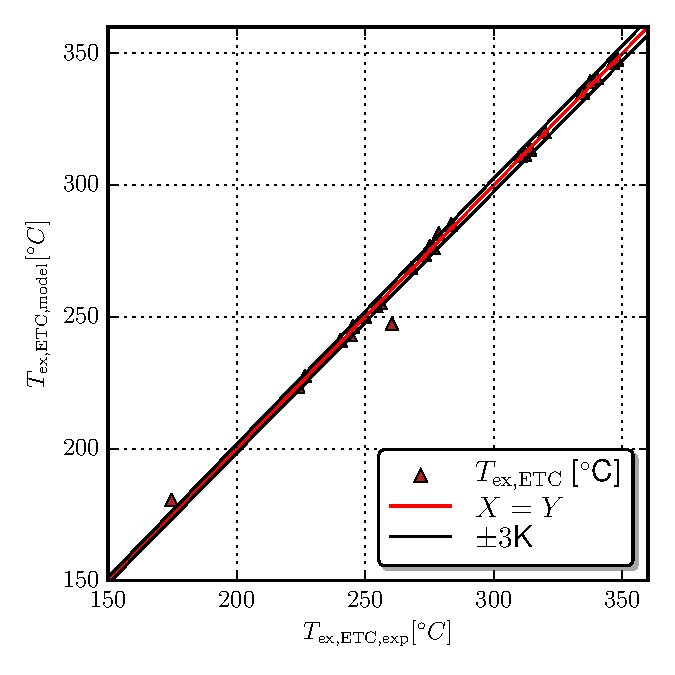
\includegraphics[width=0.6\textwidth]{Figures/StSt_Validation.pdf}
	\caption{Parity plot for the ETC model outlet temperature compared against the experimental steady-state data.}
	\label{fig:SF_ModModel}
\end{figure}
%
%
\subsection{Results:Dynamic validation}  \label{Sec:DynamicValidation}
%
The SF Modelica model was run on Dymola2017. The Differential Algebraic System Solver (DASSL) \cite{Petzold1983} was selected as numerical solver, setting the relative tolerance to 10$^{-4}$. In order to increase the model robustness and decrease the computational time, the measured variables imposed as exogenous inputs to the SF model, see Table \ref{Tab:SF_Inputs}, are approximated by a spline function in the Modelica/Dymola simulation environment.\\
In Figure \ref{fig:SF_ModRes_Zoomed}, the simulated ETC outlet temperature is plotted versus time and compared against the measured data for each of the three performed dynamic experiments. On the left abscissa the measured ETC inlet and outlet temperatures and the simulated ETC outlet temperature are plotted versus time. On the right abscissa the DNI and oil mass flow rate, $\dot{m}_\mathrm{wf}$, normalized with respect to the maximum value reached during the day are reported. For all the plots it is possible to see how the DNI was characterized by variation smaller than 2\%.\\

In Figure \ref{fig:SF_ModRes_Zoomed}a the results for the MFE experiments and simulation results are reported. Starting from a steady-state condition two consecutive steps of the same magnitude upwards and downwards were imposed to the pump rotational speed at t=450 seconds and t=1430 seconds respectively. As the pump rotational speed was raised at t=450 seconds, the velocity and pressure of the fluid in the high pressure line increased. This resulted in an oil mass flow rate, $\dot{m}_\mathrm{wf}$, increment of about 40\% in around 60 seconds. The increase in oil mass flow rate caused a drop in the temperature at the outlet of the ETC, $T_\mathrm{ex}$. The $T_\mathrm{ex}$ drop was registered at around t=500 seconds, 50 seconds after the oil mass flow rate started changing. This was due to the time required by the oil mass flow rate to reach the outlet of the 70.8 m long receiver tubes. During the experiments the ETC inlet temperature, $T_\mathrm{su}$, was maintained constant  by manually manipulating the air cooler and electrical heaters power. 
When the oil mass flow rate was changed upwards, as $T_\mathrm{su}$ was expected to decrease the air cooler power was 
decreased and the electrical heaters power was increased manually, causing a small bump of 2~K in the temperature as it is shown in Figure \ref{fig:SF_ModRes_Zoomed}a.  
The same phenomena in the opposite direction took place when the pump speed was decreased. 
The ETC outlet temperature presented a symmetrical trend for the upwards and downwards oil mass flow rate change. The SF model was able to well predict the experimental trend both for the upward and downward steps and was characterized by a time constant slightly smaller than the real system.\\

In Figure \ref{fig:SF_ModRes_Zoomed}b the TE experiments and simulation results are reported. Starting from a steady-state condition the air-cooler was turned off at t=900 seconds. This resulted in an increase of $T_\mathrm{su}$ and a consequently growth of $T_\mathrm{ex}$ delayed by around 100 seconds due to the time required by the oil mass flow to travel through the tube receiver. The shut-down of the oil-cooler did not allow to impose a step to $T_\mathrm{su}$ which increased with a slow first order trend. The large time constant characterizing $T_\mathrm{su}$ defined the change of the outlet ETC temperature. The SF model was able to correctly predict the experimental results including  the delay characterizing the $T_\mathrm{ex}$ change.\\

Finally, in Figure \ref{fig:SF_ModRes_Zoomed}c, the SBE experiments and simulation results are shown. Starting from a steady-state condition the ETCs were defocused at t=360 seconds, such that no solar radiation was reflected to the receiver tubes. This caused a sudden decrease of $T_\mathrm{ex}$ which reached the $T_\mathrm{su}$ value in about 200 seconds. The ETCs were focused again at t=650 bringing $T_\mathrm{ex}$ back to its initial value. During the experiment the oil mass flow rate and $T_\mathrm{su}$ were kept constant. The latter was maintained at its initial value by manually manipulating the power of the two electrical heaters installed after the pump. This resulted in a small bump of less then 4~K after the collectors were focused at t=700 seconds. The $T_\mathrm{ex}$ was characterized by a symmetrical behaviour during the focusing-defocusing experiments, as the thermal energy losses were relatively small. The SF model was able to replicate the trend and presented a slightly smaller time constant than the real system.\\
Overall it can be concluded that the SF Modelica model was capable of predicting the physical phenomena characterizing the real system behaviour during the three performed experiments and can be considered validated.

In Figures~\ref{fig:SF_ModRes_First3Days} - \ref{fig:SF_ModRes_Second3Days}  the simulation and experimental results for all of the six days of the experimental campaign are reported. In Figure ~\ref{fig:SF_ModRes_First3Days} - \textit{Day I}, the three minutes time over which the $\epsilon_\mathrm{un}$ parameter was optimized are highlighted by two vertical black dotted lines. During Day 6, continuous changes were imposed to the PTTL facility to test the model during highly variable conditions. As shown in Figure~\ref{fig:SF_ModRes_Second3Days} - \textit{Day VI}, the model is able to correctly predict the collector outlet temperature despite the  extreme variations.

%
\begin{figure}[h!]
\centering
\includegraphics[width=0.7\textwidth]{Figures/_MassFlowChange.pdf}
\caption{Simulation and experimental results plotted versus time for: a) MFE - Mass flow change experiment  b) TE - inlet ETC temperature change experiment c) SBE - solar beam radiation change experiment. The measured inlet and outlet ETC temperatures and the outlet SF model temperature are plotted on the left abscissa. The normalized DNI and oil mass flow rate values are plotted on the right abscissa.}
\label{fig:SF_ModRes_Zoomed}
\end{figure}
%
%
\begin{figure}[h!]
\centering
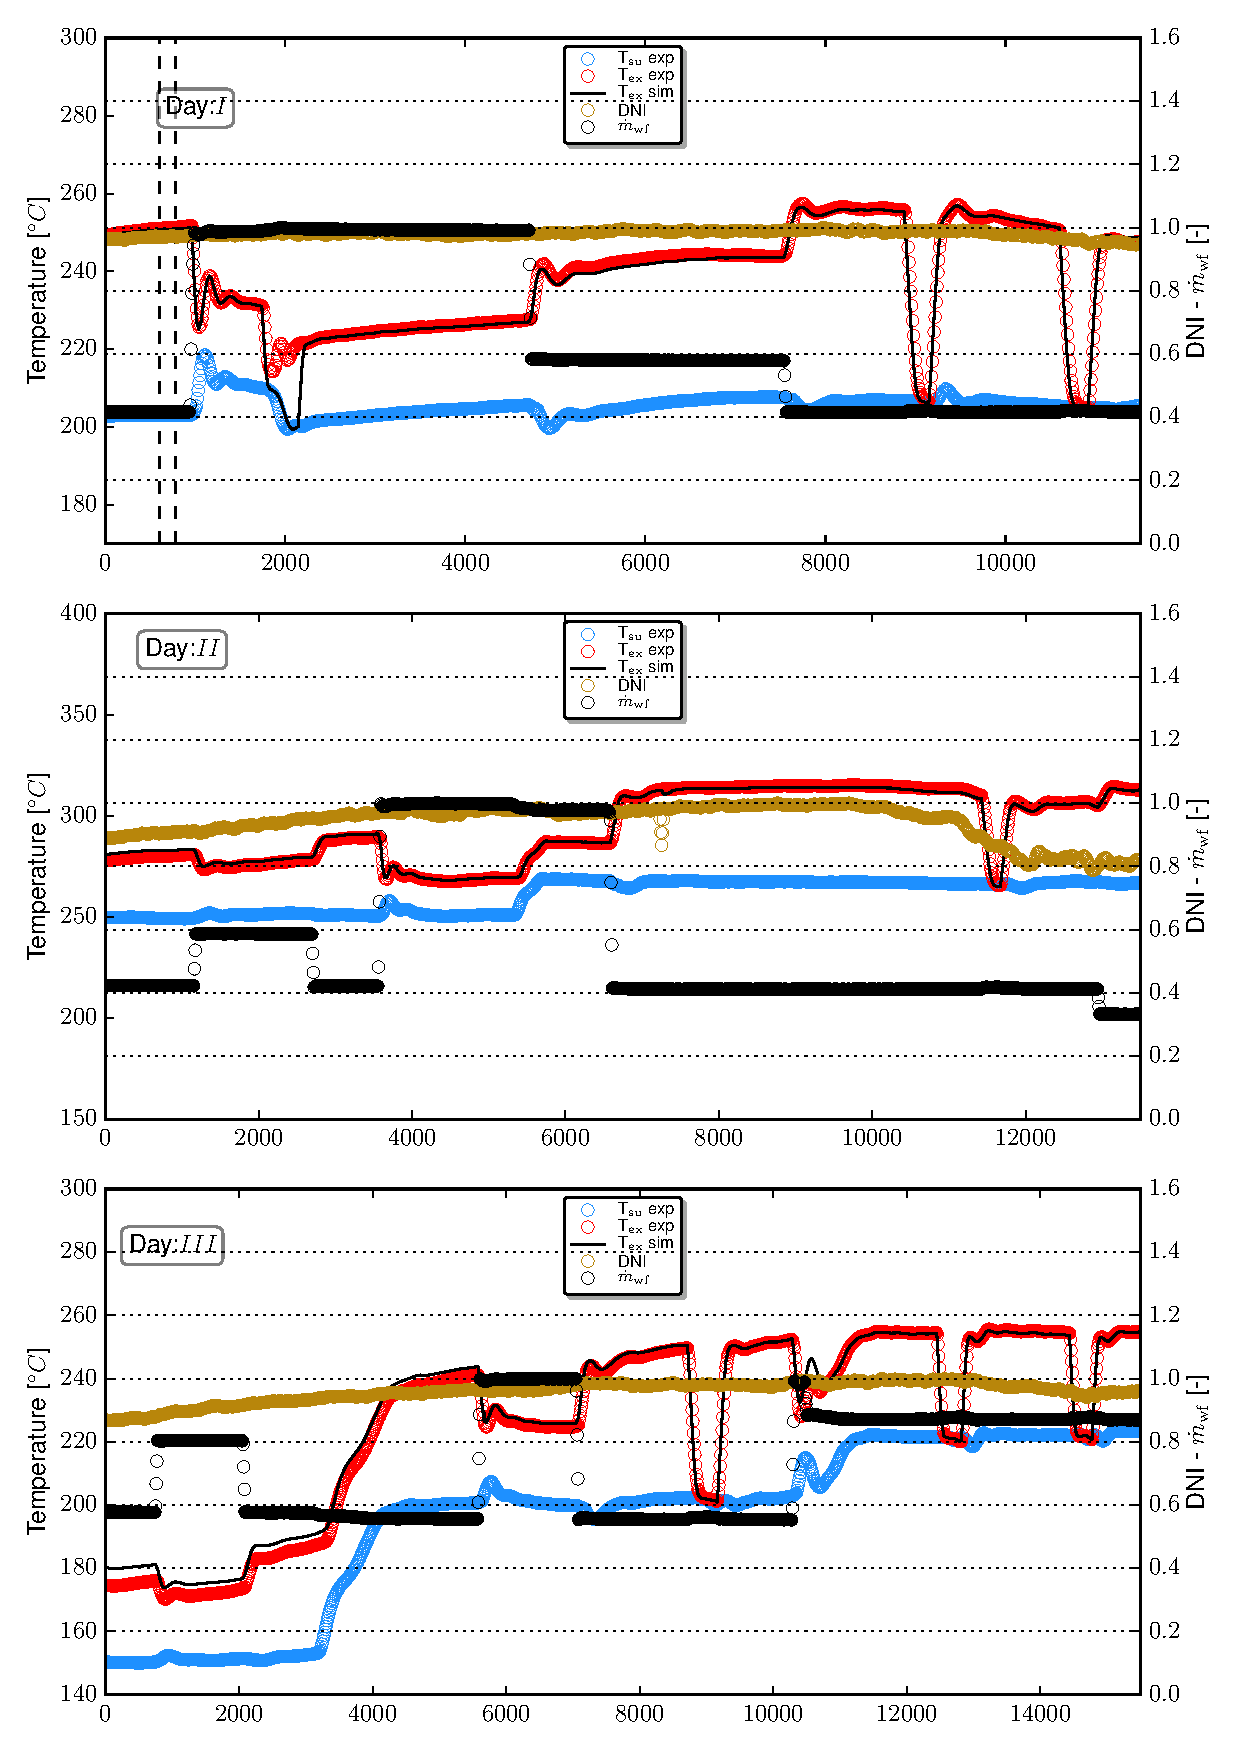
\includegraphics[width=0.8\textwidth]{Figures/_FirstThreeDays.pdf}
\caption{Simulation versus experimental results for the first three days of the experimental campaign plotted versus time. }
\label{fig:SF_ModRes_First3Days}
\end{figure}
%
%
\begin{figure}[h!]
	\centering
	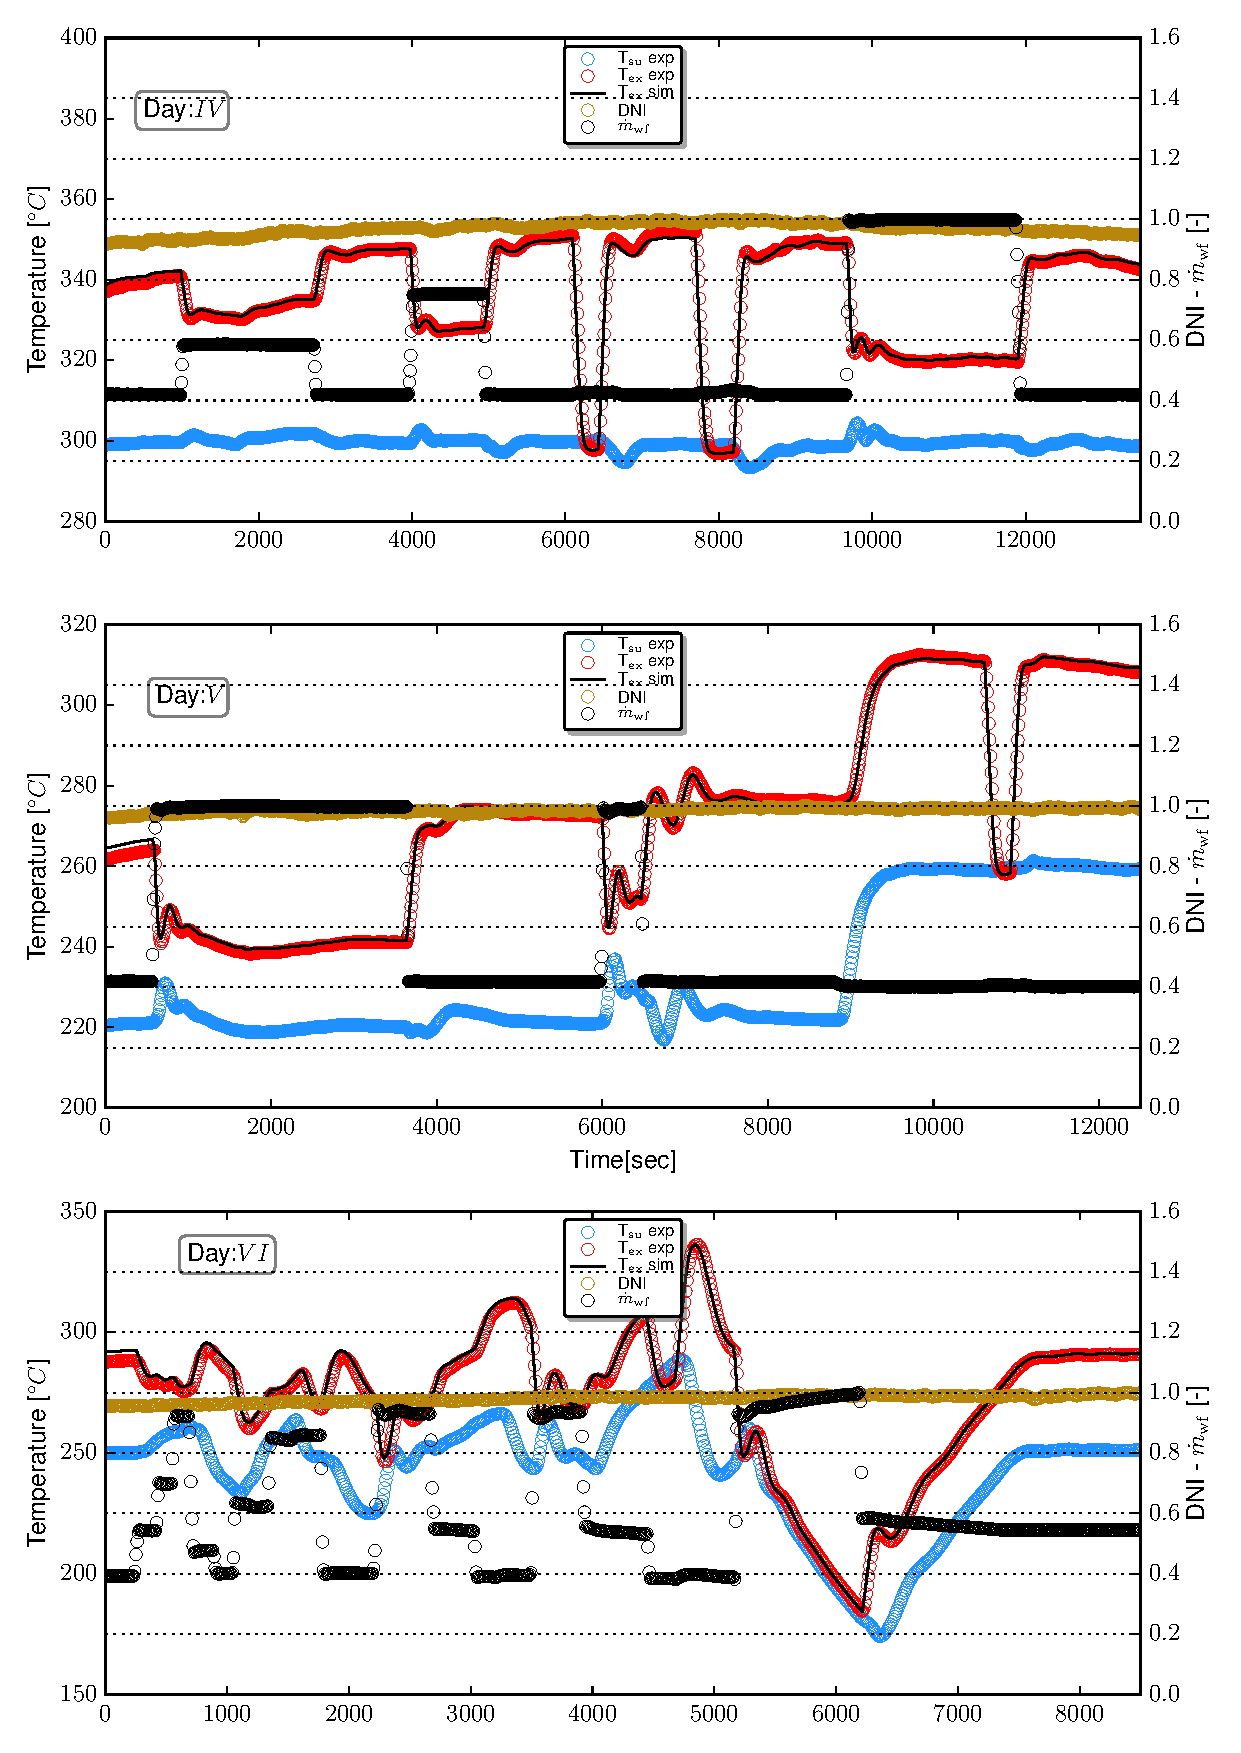
\includegraphics[width=0.8\textwidth]{Figures/_SecondThreeDays.pdf}
	\caption{Simulation versus experimental results for  the second three days of the experimental campaign plotted versus time. }
	\label{fig:SF_ModRes_Second3Days}
\end{figure}
%
\clearpage
%
\subsection{Simulation tool} \label{Sec:SimTool}
%
A simulation application of the developed PTC model was built as a tool to reproduce the results presented in section \ref{Sec:Validation}. This application can be also useful for studying the system dynamics and to evaluate the influence of the model parameters. This simulator is open source and is freely available at \url{https://ciemat-psa.gitlab.io/surf-simulator/projects/EuroTrough}. Currently, there are binary versions for Linux and Windows platforms.

Figure~\ref{fig:SimTool} shows some screenshots of the application. The application includes the Modelica model exported following the Functional Mock-up Interface (FMI) standard, input files, experimental results, diagrams and documentation about the model and experiments.

\begin{figure}[h]
	\centering
	\begin{subfigure}[t]{0.48\textwidth}
		\centering
		\includegraphics[width=\textwidth]{Figures/EuroTrough-surf1.png}
		\caption{PTC experimental and simulated outlet temperatures}
		\label{fig:SimTool1}	
	\end{subfigure}
	\begin{subfigure}[t]{0.48\textwidth}
		\centering
		\includegraphics[width=\textwidth]{Figures/EuroTrough-surf2.png}
		\caption{Summary table}
		\label{fig:SimTool2}
	\end{subfigure}
	\begin{subfigure}[t]{0.48\textwidth}
		\centering
		\includegraphics[width=\textwidth]{Figures/EuroTrough-surf3.png}
		\caption{Fluid, tube and glass temperatures in each CV}
		\label{fig:SimTool3}	
	\end{subfigure}
	\begin{subfigure}[t]{0.48\textwidth}
		\centering
		\includegraphics[width=0.9\textwidth]{Figures/EuroTrough-surf4.pdf}
		\caption{Diagram}
		\label{fig:SimTool4}
	\end{subfigure}	
	\caption{EuroTrough simulation tool.}
	\label{fig:SimTool}
\end{figure}

In the main window menu, one of the six operating days, discussed in section~\ref{Sec:DynamicValidation} (\textit{Day I} - \textit{IV}), can be selected. Model parameters (see Table \ref{tab:SF_parameter}) are shown in a tree structure on the top left side, where the user can change their default values. Simulation controls are shown on the bottom left side. When the simulation is completed, a particular time instant can be selected by manipulating the simulation bar. Inputs and results are shown on the right top side. Several tabs organize this information. A summary in a table, displays some variables' values for a particular point in time (see Figure~\ref{fig:SimTool2}). Simulation results are also compared against experimental data in line plots (see Figure~\ref{fig:SimTool1}). A bar plot presents the fluid, tube and glass temperatures for a particular point in time in each CV (see Figure~\ref{fig:SimTool3}). On the bottom right side, there are three tabs, the \textit{authors} tab provides information about the authors, the \textit{resources} tab can include documents, pictures and external links and the \textit{model \& experiment} tab provides additional information. There is a thumbnail in this tab. A diagram of the process is displayed in another window when the thumbnail is clicked. This diagram can graphically describe the process and displays information about a particular point in time of the simulation (see Figure~\ref{fig:SimTool4}).

Plots have contextual menus which allow the user to change their appearance and configuration. Additionally, results in plots can be exported as data or graphs to files or the clipboard.

%
\section{Discussion} \label{Sec:Disccusion}
%
This work aims at proposing a tool to analyse the unsteady operations of parabolic through collectors, with a special
attention to the following characteristics:
%
\begin{itemize}
	\item Satisfactory accuracy for engineering scopes
	\item Low computational time
\end{itemize}
%
The SF model is based on the finite volume method, characterized by a trade-off between model accuracy and computational time: increasing the number of CVs leads to better accuracy but negatively affects
the computational effort.

In order to investigate the effect of the level of discretization on the performance of the SF model when compared to the experimental results a parametric analysis was performed. The SF model, discretized with a number of control volumes (CVs) varying from 1 to 50,  was simulated to replicate the  experimental data of Day $IV$, see Figure \ref{fig:SF_ModRes_Second3Days}. The results are displayed in Figure \ref{fig:SF_ModRes_ParAnalysis}a where the simulated SF outlet temperature for the different levels of discretization is plotted versus time and compared against the measured experimental data on the left abscissa. On the right abscissa the nominal DNI and oil mass flow rate are plotted. Overall as the level of discretization increased the SF outlet temperature got closer to the measurements data. From 10 to 50 CVs the improvement in model accuracy was negligible. On the other hand the 5 CVs and 1 CVs SF model presented a slower time constant compared to the real system and were not able to properly predict the different undershoot and overshoot characterizing the measured outlet ETC temperature when the boundary conditions where changed, e.g., step change in the mass flow (MFE) or defocusing-focusing (SBE).\\
In Figure \ref{fig:SF_ModRes_ParAnalysis}b the percentage computational effort (PCE) defined in equation \ref{eq:PCE} as the ratio of the computational time (Time$_\mathrm{Comp}$) with respect to the simulated real time ($\mathrm{Time}_\mathrm{Real}$), is plotted for each simulation result. All the simulation results were characterized by a much shorter time compared to the real simulated time. This is related to the remarkably simple simulation framework on which the modelling results were based on (see section \ref{subsec:SF_model}). 
%
\begin{equation}
\mathrm{PCE} = \frac{\mathrm{Time}_\mathrm{Comp}}{\mathrm{Time}_\mathrm{Real}} \cdot 100
\label{eq:PCE}
\end{equation}
%
The computational time increased exponentially with the increase of number of CVs with the 1 and 5 CVs SF models being one order of magnitude faster than the higher discretized model.\\
In order to assess the discrepancy between the different CVs discretization levels, the total energy absorbed by the thermal oil in the ETC collectors, $E_\mathrm{wf}$,  was computed as the integral of the thermal power over the simulated time, around 4 hours, and compared with respect to the 50 CVs model which was taken as a reference. The percentage relative error $\bar{\epsilon}$ for each SF model was computed as:
%
\begin{equation}
\bar{\varepsilon}(k) = 100 \cdot \frac{|E_\mathrm{wf,50CVs} -E_\mathrm{wf,k}|}{E_\mathrm{wf,50CVs}}  \quad k \in [1,5,10,20]. 
\end{equation}
%
The results are reported in Table \ref{tab:SF_Etot}.
%
\begin{table}[h!]
  \centering
  \caption{Total energy percentage relative error for the different levels of discretization of the SF model.}
    \begin{tabular}{lc}
    \toprule
    Model & \multicolumn{1}{c}{$\bar{\varepsilon}$ [\%]}  \\
    \midrule
    SF CVs 1      & 0.5         \\
    SF CVs 5      & 0.18         \\
    SF CVs 10     & 0.08          \\
    SF CVs 20     & 0.03          \\   
    \bottomrule
    \end{tabular}%
  \label{tab:SF_Etot}%
\end{table}%
%
As it possible to see, the overall percentage relative error on the total energy absorbed by the fluid over 4 hours of simulation with respect to the 50 CVs SF reference model was negligible for all the tested levels of discretization.\\

%1 - 5 - 10 - 20 
% 0.50323002464612376, 0.1887974297686737, 0.08694895129959232, 0.03231713606505187
\begin{landscape}
\begin{figure}[h!]
\centering
\includegraphics[height=0.95\textheight]{Figures/_SF_NodesParaALL.pdf}
\caption{Simulation results versus the experimental results for each full day of the experimental campaign. PCE: percentage computational effort.}
\label{fig:SF_ModRes_ParAnalysis}
\end{figure}
\end{landscape}
%
%
%

%


%
\section{Conclusions} \label{Sec:Conclusions}
%
This paper presents a dynamic model included in the ThermoCycle modelica library for the modelling of parabolic through collectors. The proposed model is validated against experimental data acquired on the PTTL facility at the Plataforma Solar de Almer\' ia (PSA), Spain. Steady-state and dynamic experimental data were obtained at different operating conditions by varying the pump rotational speed, the heater and cooler set-points and by focusing-defocusing the collectors. A first validation is performed against 24 steady-state data points. A second dynamic validation is carried out with 3 sets of experiments by varying the oil mass flow rate (MFE), the oil inlet temperature (TE) and the solar beam radiation (SBE).
The main outcomes of this study are reported hereunder.
%
\begin{itemize}
\item The steady-state validation shows a good agreement between experimental and simulated temperature at the outlet of the collectors. Most of the data are reproduced with an accuracy below 3$^{\circ}$C. For temperature below 200$^{\circ}$C, the temperature is predicted with a  4$^{\circ}$C error.
\item The simulation results obtained for the oil mass flow   (MFE), the oil inlet temperature   (TE) and the solar  beam radiation (SBE) experiments showed a good overlap with the experimental results. The developed solar field model structure proves to be effective to predict the dynamic of a real line of solar collectors.
%
%Based on these analyses the following conclusions can be drawn:
%\begin{itemize}
%\item The SF model structure proved effective to simulate parabolic trough collectors systems when subjected to change in the inlet mass flow rate (MFE), the inlet temperature (TE) and to variation of the solar beam (SBE).
%\item A minimum discretization level of 20 CVs is recommended if the ETC outlet temperature has to be precisely predicted, e.g., the  SF model is used as a reference to develop and test model based control strategies. 
%\item A single CVs is sufficient if the performance of the ETC collectors are analysed on a daily or longer basis. This approach allows to significantly decrease the computational time while maintaining a satisfying degree of accuracy.
%\end{itemize}
%
\item A minimum discretization level of 20 CVs was found to be a good compromise between model accuracy and simulation speed if the ETC outlet temperature had to be precisely predicted, e.g., the  SF model is used as a reference to develop and test model based control strategies.
%
\item In light of the obtained results a lumped SF model is recommended if the performance of the ETC collectors are analysed on a daily or longer time frame. This approach allows to significantly decrease the computational time while maintaining a satisfying level of accuracy.
%
\item An simulation tool has been built to reproduce the dynamic validation results presented in this paper. The tool is open-source and can be used as a reference for modelling parabolic through collectors.
\end{itemize}
%
It was proven that the modelling approaches adopted led to satisfactory results for the simulation of parabolic trough collector systems. The proposed solar collector model together with the test cases is released as open-source and is available in the latest version of the ThermoCycle library. It should be noted that the model is not suitable for the simulation of start-up or shut-down of the collectors, as the proposed finite volume approach does not handle zero flow conditions.
%
%
%
\section{Acknowledgements}
%
The results presented in this paper have been obtained within the frame of the SFERA II project. These financial supports are gratefully acknowledged.
Furthermore, the authors want to thank the financial support received from the BRICKER project (www.bricker-project.com). This project has received funding from the European Union’s Seventh Framework Programme for research, technological development and demonstration under grant agreement No 609071. The information reflects only the author’s view and the Commission is not responsible for any use that may be made of the information it contains.

%
\clearpage
\bibliographystyle{model3-num-names}
\bibliography{Solar}


\end{document}
\endinput



